\section{Operationalization}
\todo{discuss why discontinuity only at lower cardinalities}
\todo{describe experimental setup: number of queries, dbmses, etc}
In this model, we consider plan-operator discontinuity as an independent 
variable in that the occurrences of sub-optimality is not necessarily dependent
on the presence of discontinuous plan-operators, such as a hash-join
operator. However, we predict that when discontinuous plan operators
selected, they may introduce complexity to query optimization especially
at the point where discontinuity is observed. This is because the performance
of such operators is sensitive to the input size. An inaccurate estimation
in the plan statistics may lead the optimizer to keep a plan that
starts to require additional passes over the input data, which could be
significantly less efficient than an alternative plan. Therefore,
we consider such discontinuous plan operators to have positive effects
on the sub-optimality phenomenon.

To study the presence of discontinuous plan operators, more importantly,
to quantify their effects for the later-performed linear regression,
we designed a simple discontinuity-identification technique. We present
an example to illustrate how discontinuity, which is observed in the hash-join
operators for a particular query, is identified.

\begin{figure}[th]\centering
\includegraphics[width=0.40\textwidth]{figures/discontinuity.eps}
\caption{An Example of Discontinuous Plan Operators (Hash-Join)
\label{fig:discontinuity}}
\end{figure}

Figure~\ref{fig:discontinuity} presents for a single query
\shorten{({\em query4}, exhaustive-10q-1, oracle)}, as the cardinality
increase, the {\em cost} of all the hash-join operators utilized in each
plan at a particular cardinality. Each distinct color depicts an individual
hash-join operator.
Note that we ensure the plan-operator equality by examining first the
equality of the entire plans. In other words, if two plans are identical,
then the hash-join operator that appears at the same position in these two
plans are inherently identical. As shown by this figure, the hash-join shown
in cyan has two discontinuous points, both appearing below cardinality
200K. The hash-join in yellow has one discontinuous point.

To systematically identify such discontinuous instances, we employ a simple
slope-based measurement. According to the monotonic characteristic
of a plan operator, it is expected that as the input size increases,
the cost of executing the operator will steadily increase. In the case
of hash-join operator, since its performance is linear to the input size,
we expect that the increase in the execution cost can be characterized by
some slopes that are stable and consistent.
Therefore, by identifying a sudden change in the slope, we can effectively
spot the cardinality at which an operator becomes discontinuous.

Formally, we compute the slope between each pair of consecutive cardinalities
as the following.\\
$S_{card} = (C_{card + 10K} - C_{card}) / 10K$\\

\todo{Sabah will change the following discussion to distribution analysis}
As a result, a series of slope values are computed.
We then compute the standard deviation of all the slope values. Although
there are briefly four classes of operator cost, as indicated by the cyan
hash-join operator in Figure~\ref{fig:discontinuity}, (corresponding to four
groups of slope values), the major variance is introduced by the discontinuous
points. Hence, by identifying the slope values that are greater than one
standard deviation over the average value, the discontinuous can be effectively
discovered. For this particular example, we assign a value {\em 3} to this
variable (number of gaps) since there are three discontinuous points.

\todo{Rick: please read}\\
We operationalize discontinuity in our model by counting and summing the
number of discontinuous operators. Specifically, in the example shown in
Figure~\ref{fig:discontinuity}, two distinct hash-join operators, represented
as the cyan and yellow curves, respectively, are discontinuous. Hence the
value of discontinuity of this query is two. We choose such a
operationalization metric based on the following considerations.

\begin{itemize}
\item{} Due to the sensitivity of the performance of discontinuous plan
operator w.r.t. the operator-cost estimation, such operators can be a major
factor to the presence of suboptimality. Hence, the more discontinuous plan
operators are employed by a query, the higher chance suboptimality will be
observed for this query.

\item{} We do not particularly weight the series of cardinalities, with which
query plans are collected, differently. One might argue that discontinuous
operators that appear at higher cardinalities should have more significant
performance impact than those appearing at lower cardinalities.
We consider an operator to be discontinuous for all the cardinalities, where
this operator is observed, if it is discontinuous for at least once.
Hence the actual values of the cardinalities are not relevant to this metric.

\item{} Furthermore, we do not count the total number of instances of
discontinuity of each plan operator. For instance, the operator represented by
the cyan curve in Figure~\ref{fig:discontinuity} has two discontinuous
instances. The reason is that the frequency of discontinuity for a particular
operator is dependent on a number of factors. For instance, the position
of an operator, whether it is high-up in the plan tree or at the bottom,
may result in more or less occurrences of discontinuity for this operator.
In our study, we consider suboptimality at query plan level rather than within
a plan. In addition, extremely frequent occurrence of discontinuity is not
observable since discontinuity is determined largely by the input-size
estimation of a particular operator. Hence given the gradual change of the
cardinalities in our experiments, no more than three instances for an
individual operator are observed. Therefore, we exclude the in-plan
discontinuity-frequency measurement and focus on the occurrences of
discontinuous operators themselves.
\end{itemize}

\todo{later we will investigate non-linear operators..?}

\todo{The rest of the section below  should go before description of 
discontinuous operators}
An experiment was used to test the model. We selected five relational
DBMSes that are representative of the relational DBMS the market.

The experimental specification configures 600 randomly generated
queries. Each query
is a select-project-join-aggregate query, with a few attributes in the
SELECT clause, a few tables referenced in the FROM clause, a few
equality predicates in the WHERE clause, and zero or more aggregate
functions. As such some of the complexities
mentioned by Kabra and DeWitt~\cite{kabra98}, such as
user-defined data types, methods, and operators, are not considered.
The queries were generated
by a simple algorithm, the pseudo-code for which is shown in
Figure~\ref{alg:querygen}.

The query generator has \todo{is it four? Rui/Matt, could you please put
in the function names for Aggregates} 
main components, which are {\tt
  generateSelectClause()}, {\tt generateFromClause()}, {\tt
  generateWhereClause()} and {\tt generateGroupByClause()}. 
\todo{Q: does primary key have its own function?}
The select clause will contain from one to four
columns\c2j{}{, hence, an average of 2.5 columns}. The number of
correlation names
in the FROM clause varied from one to four, with duplication of tables
allowed (duplicate table names within a from clause implies a self-join).
In the queries that were generated, from one to four unique tables were
mentioned in the FROM clause. Somewhat fewer tables were mentioned than the
number of correlation names, as the presence of self-joins reduced the
number of unique tables named by the queries.

In {\tt generateWhereClause()}, in which all the joins will appear, we make
sure that Cartesian products are
eliminated\c2j{.}{(\verb.cartesianPossible="false".)}  We do this by
connecting all the correlation names that appear in the FROM statement via
comparisons on random columns. In this case, the comparisons are all
equality operators. To ensure that the queries are as simple as possible, we
do not include any additional predicates in the WHERE clause.  \c2j{}{This
  is realized by setting the attributes {\tt maxIsAbsolute} to {\tt true}
  and {\tt complexUsePercentage} to {\tt 100}.  Basically, ``complex''
  predicates eliminate the Cartesian product, and by setting complex
  predicates as ``absolute,'' no additional predicates are included except
  for those which are necessary for eliminating Cartesian product.} Also for
simplicity, we do not include disjunctions nor negations.

In the \todo{Correct name: generateGroupByClause}, where the aggregate
functions and
grouping occurs, the presence or absence of a group by clause is
recorded. We expect the
complexity of the query to increase when the first aggregate function
is introduced. However,
additional aggregate functions in the same SELECT clause will not add
significant complexity since
they share the same grouping function.

We are interested in predicting the behavior of DBMSes through our
model. Therefore, we vary the cardinality from 2M (maximum) to
100K (minimum), in increments of 10K. For one of the DBMSes that was
slower than the others and was timing out for the majority of the
queries
when run between 100K and 2M, we reduced the size of the tables and
varied the cardinality from 200K (maximum) to 10K (minimum), in
increments of 1K.

We identify the cardinalities where the plan selected changed (change
point) in a single iteration increment.
At the cardinality before the change (higher) and after (lower), we
run and time the query executions 10 times each.
We reduce the runtime by timing of other processes (identified by
psdiff) and remove any executions that had phantoms or stopped processes.
We then compare the average runtimes
and standard deviations at the cardinality just before the change
point (n-1) and at the change point (n). The query is said to be suboptimal
$if avg_{n-1} + 0.5 * stddev_{n-1} <= avg_n - 0.5 * stddev_n$.

\todo{Rick, please check}Suboptimality is coded as follows:
a) Not suboptimal, i.e., $0 IF avg_{n-1} + 0.5 * stddev_{n-1} > avg_n -
0.5 * stddev_n ;$
b) Low suboptimality, i.e., $1 IF avg_{n-1} + 0.5 * stddev_{n-1} <=
avg_n - 0.5 * stddev_n$, and
$avg_{n-1} + 1.0 * stddev_{n-1} > avg_n - 1.0 * stddev_n$;
c) Moderate suboptimality, i.e., $2 IF avg_{n-1} + 1.0 * stddev_{n-1}
<= avg_n - 1.0 * stddev_n$, and
$avg_{n-1} + 1.5 * stddev_{n-1} > avg_n - 1.5 * stddev_n$;
b) High suboptimality, i.e., $3 IF avg_{n-1} + 1.5 * stddev_{n-1} <=
avg_n - 1.5 * stddev_n$


One of the constructs that
our model predicts ``number of operators in the DBMS'' is a factor
that will impact suboptimality. By number of operators,
we mean the number of operators available for selection, projection,
join and aggregate functions. As the number
of operators available increases, the complexity of the optimizer
increases because it has to choose between more
operators, and hence the probability of suboptimality increases.

Not all operators available in a DBMS are considered by the optimizer.
For example, for joins, nested loop is rarely considered
if there are other operators available for joins. However, in
proprietary DBMSes, we cannot capture the latent variable number of
operators
considered. Therefore, we try to approximate this by counting ``Number
of operators observed'' chosen across plans for each query.

The overall effect of the primary key moderator is to reduce the strength 
of the relationship between the number of correlation names in from to 
CEPS and subopt and from presence of aggregates to CEPS/supopt.

More specifically, if primary key is not on 
a) any of the joining columns for tables (or there is only one table 
involved in the query), then presence of primary keys will NOT have any 
impact on the relationship of ``\# of correlation names in FROM'' (OR from 
``\# of self joins'') to any other variable (No moderating effect)

b) any of the Grouping columns in aggregate function and is not on any 
columns involved in the joins, then presence of primary keys will NOT 
have any impact on the relationship from "Presence of aggregates" to 
any other variable.

c) any of the Grouping columns in aggregate function but is on the 
columns involved on the joins then the presence of primary key will 
not have any moderating effect on the relationships from presence of 
aggregates to CEPS/supopt

If primary key is on 
d) one side of a join condition, for a subset of the joins, the 
primary key will have less of an impact on the relationship between 
"\# of correlation names in FROM" and Suboptimality compared to when 
all of the columns had a primary index defined on them. 

e) one side of a join condition, for all the joins, the primary key 
will have more of an impact on the relationship between "\# of correlation 
names in FROM" compared to when some of the columns had a primary index 
defined on them (on one side of the join condition). 

f) both sides of a join condition, for a subset of the joins, the primary 
key will have more of an impact on the relationship between "\# of 
correlation names in FROM" and Suboptimality compared to when none of 
the columns had a primary index defined on them and more compared to d) 
primary key is on one side of the join condition, for a subset of the 
joins (assuming that d) was similar in number of total joins, and had a 
similar number of joins involving primary keys). 

g) both side of a join condition, for all of the joins, \# of correlation 
names will not affect plan space complexity / suboptimality. 

h) If primary key is on a subset of SELECT /GROUP BY columns in aggregate, 
then the presence of primary keys will have more of an impact on the 
relationship "Presence of aggregates" to Suboptimality vs. no primary 
key on any of the columns in GROUP BY clause.

i) If primary key is on all the columns of SELECT /GROUP BY columns in 
aggregate, then presence of primary keys will have a very strong 
moderating effect: "Presence of aggregates" will have no impact on 
Suboptimality. 

The aggregate is generally done after all the joins are completed; 
therefore, the presence of primary keys on non-GROUP BY columns should 
not impact the relationship between presence of aggregates and suboptimality. 

\shorten{To estimate the error a DBMS makes in estimating the cost of a plan,
we use a variable called ``Flutter'' that counts the number of times a
plan repeats
in non contiguous blocks \todo{Rick, please check}
Flutter per query = (Max(Count(planID involved in change point)) - 1}
